\pagebreak

\hthree{REST vs. SOAP}

SOAP (Simple Object Access Protocol) ist ein Netzwerkprotokoll, welches sich auf XML-Repräsentation der Daten und auf Internet-Protokolle stützt. Es ist neben der REST-Architektur eines der meistverbreiteten Protokollen im Bezug zu Web-Services. Was die Unterschiede zwischen REST und SOAP sind und in welchen Fällen welche Architektur bevorzugt werden sollten wird in diesem Kapitel beschrieben. 

\begin{figure}[H]
    \centering
    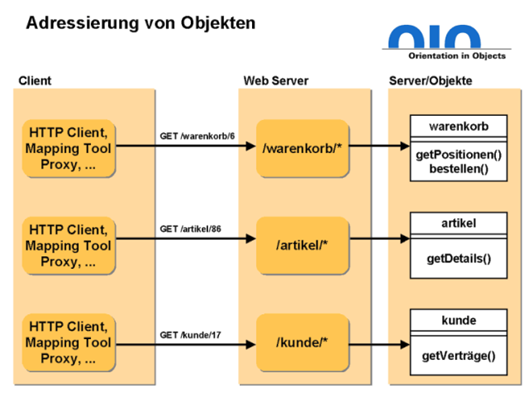
\includegraphics{media/REST/restcomm.png}
    \caption{REST-Kommunikation \cite{RestSoap}}
\end{figure}

Auf der Abbildung sieht man den Zugriff auf Ressourcen bei einer REST-Anwendung. Dabei kann auf den Warenkorb, den Artikel und auf den Kunden über die jeweilige URI zugegriffen werden. 

\begin{figure}[H]
    \centering
    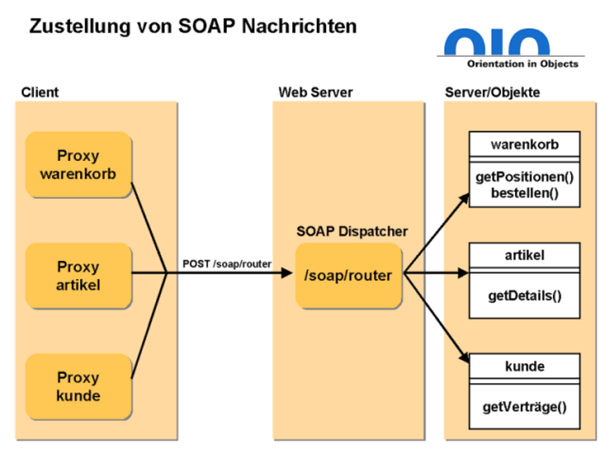
\includegraphics[width=0.9\textwidth]{media/REST/soapcomm.png}
    \caption{SOAP-Kommunikation \cite{RestSoap}}
\end{figure}

Bei SOAP wird jedoch nicht direkt auf die Ressource zugegriffen, sondern über einen sogenannten Dispatcher. Alle Aufrufe sind somit POST-Requests an dieselbe Adresse. Der Dispatcher kümmert sich dann um die weitere Verarbeitung der Daten. Die Implementierung des Dispatchers erfolgt üblicherweise über ein CGI-Skript. Ein wesentlicher Unterschied zu REST ist also die Art und Weise, wie auf Ressourcen zugegriffen wird. REST bietet mit den verschiedenen URIs die Möglichkeit jede einzelne Ressource anzusprechen. Grundsätzlich ist SOAP ein Baukasten, mit dem ein Entwickler sein eigenes Anwendungsprotokoll entwickelt. Das Protokoll, dass der Entwickler daraus definiert, beschreibt genau, wie eine Anfrage, beziehungsweise eine Antwort auszusehen hat. Dadurch wird die Möglichkeit zur Erweiterung des SOAP-Interfaces praktisch abgeschafft. Wenn der Server zusätzliche Informationen liefern will, muss er das über ein komplett neues Interface tun. REST jedoch ermöglicht beispielsweise die Mitlieferung von zusätzlichen Daten, ohne dass das Web-Interface verändert werden muss. \cite{RestSoap}